\documentclass[12pt, a4paper, onecolumn, oneside, final]{report}
\usepackage[latin1]{inputenc}
%\usepackage[bahasa]{babel}
\usepackage{amsmath}
\usepackage{amsfonts}
\usepackage{amssymb}
\usepackage{tocloft}
\usepackage[left= 3.5cm,right=3cm,top=3cm,bottom=3cm]{geometry}
\usepackage{indentfirst}
\usepackage{amsmath,amssymb,amsfonts,amsthm}
\usepackage{array}
\usepackage{caption}
\usepackage{wrapfig}
\usepackage{graphicx}
\usepackage{varwidth}
\usepackage{float}
\usepackage{indentfirst}
\usepackage{textcomp}
\usepackage{lmodern}
\usepackage{enumerate}
\usepackage{tabularx}
\usepackage{microtype}
%\usepackage[framed]{matlab-prettifier}
\usepackage{inputenc}
\usepackage{tikz}
\usepackage{xcolor,colortbl}
\usepackage{multirow}
\usepackage{times}
\usepackage{float}
\usepackage{hyperref}
\hypersetup{colorlinks=true,
	linkcolor=black,
	filecolor=black,      
	urlcolor=blue,}
%	pdfpagemode=FullScreen,}
\urlstyle{same}
\usepackage{setspace}
\usepackage{apacite}
\usepackage{enumitem}
\usepackage[labelsep=period]{caption}
%\usepackage{pbsi}
\usepackage[T1]{fontenc}
\usepackage{esint}
\usepackage{lipsum}
\usepackage{multirow}
\usepackage{ragged2e}
\usepackage[justification=centering]{caption}
%%
% Hyphenation untuk Indonesia
%
% @author  Andreas Febrian
% @version 2.02
% @edit by Ichlasul Affan
%
% Tambahkan cara pemenggalan kata-kata yang salah dipenggal secara otomatis
% oleh LaTeX. Jika kata tersebut dapat dipenggal dengan benar, maka tidak
% perlu ditambahkan dalam berkas ini. Tanda pemenggalan kata menggunakan
% tanda '-'; contoh:
% menarik
%   --> pemenggalan: me-na-rik
%


% Silakan ganti ke bahasa Inggris (\selectlanguage{english}) jika Anda merasa terlalu banyak kata bahasa Inggris yang pemenggalannya tidak benar.
\selectlanguage{bahasa}


\hyphenation{
    % alphabhet A
    a-na-li-sa a-tur
    a-pli-ka-si
    % alphabhet B
    ba-ngun-an
    be-be-ra-pa
    ber-ge-rak
    ber-ke-lan-jut-an
    ber-pe-nga-ruh
    % alphabhet C
    ca-ri
    % alphabhet D
    di-da-pat-kan di-sim-pan di-pim-pin de-ngan da-e-rah di-ba-ngun da-pat di-nya-ta-kan
    di-sim-bol-kan di-pi-lih di-li-hat de-fi-ni-si di-de-fi-ni-si-kan di-mi-li-ki
    % alphabhet E
    e-ner-gi eks-klu-sif
    % alphabhet F
    fa-si-li-tas
    % alphabhet G
    ga-bung-an ge-rak
    % alphabhet H
    ha-lang-an
    % alphabhet I
    % alphabhet J
    % alphabhet K
    ke-hi-lang-an
    ku-ning
    kua-li-tas ka-me-ra ke-mung-kin-an ke-se-pa-ham-an
    % alphabhet L
    ling-kung-an
    % alphabhet M
    me-neng-ah
    meng-a-tas-i me-mung-kin-kan me-nge-na-i me-ngi-rim-kan
    meng-u-bah meng-a-dap-ta-si me-nya-ta-kan mo-di-fi-ka-si
    meng-a-tur meng-a-rah-kan mi-lik
    % alphabhet N
    nya-ta non-eks-klu-sif
    % alphabhet O
    % alphabhet P
	pe-nye-rap-an
	pe-ngon-trol
    pe-mo-del-an
    pe-ran  pe-ran-an-nya
    pem-ba-ngun-an pre-si-den pe-me-rin-tah prio-ri-tas peng-am-bil-an
    peng-ga-bung-an pe-nga-was-an pe-ngem-bang-an
    pe-nga-ruh pa-ra-lel-is-me per-hi-tung-an per-ma-sa-lah-an
    pen-ca-ri-an pen-ce-ta-kan peng-struk-tur-an pen-ting pen-ting-nya
    % alphabhet Q
    % alphabhet R
    ran-cang-an
    % alphabhet S
    si-mu-la-si sa-ngat
    % alphabhet T
    te-ngah
    ter-da-pat
    trans-for-ma-si
    % alphabhet U
    % alphabhet V
    va-ri-an va-ri-a-si
    % alphabhet W
    % alphabhet X
    % alphabhet Y
    % alphabhet Z
    % special
}

\usepackage{amsmath,amssymb,amsfonts,amsthm}
\renewcommand{\chaptername}{BAB}
%\usepackage{setspace}

\setcounter{tocdepth}{1}

\definecolor{green}{rgb}{0.1,0.1,0.1}
\newcommand{\done}{\cellcolor{teal}done}  %{0.9}
\newcommand{\hcyan}[1]{{\color{teal} #1}}

\newtheorem{theorem}{Dalil}
\newtheorem{corollary}{Akibat}
\newtheorem{lemma}{Lemma}
\newcommand\at[2]{\left.#1\right|_{#2}}
\theoremstyle{definition}
\newtheorem{definition}{Definisi}{}
\newtheorem{example}{\textsf{Contoh}}

\newenvironment{bukti}[1][Bukti]{\noindent{\it\textit{#1. }}}
{\hspace{\stretch{1}}\rule{.5em}{.5em}}

\DeclareMathOperator{\mo}{mod\,}
\DeclareMathOperator{\ord}{ord}
\DeclareMathOperator{\fpb}{fpb}
\newcommand{\defi}{\overset{\mbox{\tiny{\sf def}}}{=}}
\newcommand{\znz}{\Bbb Z/n\Bbb Z}\newcommand{\zpz}{\Bbb Z/p\Bbb Z}
\numberwithin{equation}{chapter}

\setcounter{tocdepth}{3}
\setcounter{secnumdepth}{3}

\setlength\parindent{12.5mm}

\usepackage{blindtext}
\renewcommand\cftbeforetoctitleskip{-1cm}
 \renewcommand\cftbeforeloftitleskip{-1cm}
 \renewcommand\cftbeforelottitleskip{-1cm}
\renewcommand{\cftdotsep}{1}
\renewcommand{\cftchapleader}{\cftdotfill{\cftsecdotsep}}

\renewcommand{\contentsname}{DAFTAR ISI}
\renewcommand{\cfttoctitlefont}{\hfil\Large\bfseries\MakeUppercase}
\renewcommand{\cftchapfont}{\bfseries}
\renewcommand{\cftchappagefont}{\bfseries}
\renewcommand{\cftchappresnum}{BAB }
\renewcommand{\cftchapnumwidth}{3.7em}

\renewcommand{\cftlottitlefont}{\hfil\large\bfseries\MakeUppercase}
\renewcommand{\cfttabpresnum}{Tabel }
\renewcommand{\cfttabnumwidth}{6em}

\renewcommand{\cftloftitlefont}{\hfil\large\bfseries\MakeUppercase}
\renewcommand{\cftfigpresnum}{Gambar }
\renewcommand{\cftfignumwidth}{6em}
\renewcommand{\figurename}{Gambar}

\makeatletter
\def\ps@myPS{%
    \def\@oddfoot{\null\hfill\thepage}
    \def\@evenfoot{\thepage}%
    \def\@evenhead{\null\hfil\slshape\leftmark}%
    \def\@oddhead{{\slshape\rightmark}}}%
\makeatother

\makeatletter % default is "\newcommand\@chapapp{\chaptername}"
\renewcommand\@chapapp{\textls[40]{\MakeUppercase{\chaptername}}}
\makeatletter

\usepackage{titlesec}
% 1. Judul bab ditengah
\titleformat{\chapter}[display]
 {\normalfont\large\bfseries\centering}
 {\chaptertitlename\ \Roman{chapter}}{0pt}{\large}
% 2. Font section 12pt dan tambah titik section, so 1.1 menjadi 1.1.
\titlespacing{\chapter}{0pt}{50pt}{\baselineskip}
\titleformat{\section}[block] %tambah block untuk menampilkan format angka 
 {\normalfont\fontsize{12}{15}\bfseries}{\thesection.}{1em}{}
% 3. Font subsection 12pt dan tambah titik subsection
 \titleformat{\subsection}[block] %tambah block untuk menampilkan format angka 
 {\normalfont\fontsize{12}{15}\bfseries}{\thesubsection.}{1em}{} 
% 4. Hapus spasi setelah bab
\makeatletter
\def\ttl@mkchap@i#1#2#3#4#5#6#7{%
 \ttl@assign\@tempskipa#3\relax\beforetitleunit
 \vspace{\@tempskipa}%<<<<<< REMOVE THE * AFTER \vspace
 \global\@afterindenttrue
 \ifcase#5 \global\@afterindentfalse\fi
 \ttl@assign\@tempskipb#4\relax\aftertitleunit
 \ttl@topmode{\@tempskipb}{%
 \ttl@select{#6}{#1}{#2}{#7}}%
 \ttl@finmarks % Outside the box!
 \@ifundefined{ttlp@#6}{}{\ttlp@write{#6}}}
 
 \usetikzlibrary{shapes.geometric, arrows}
%Spasi sebelum dan sesudah judul sub bab
%\titlespacing*{\section}
%{0pt}{5.5ex plus 1ex minus .2ex}{4.3ex plus .2ex}
%\titlespacing*{\subsection}
%{0pt}{5.5ex plus 1ex minus .2ex}{4.3ex plus .2ex}

\newcommand{\listappendicesname}{DAFTAR LAMPIRAN}
\newlistof{appendices}{apc}{\listappendicesname}
\newcommand{\appendices}[1]{\addcontentsline{apc}{appendices}{#1}}
\renewcommand\cftbeforeapctitleskip{-1cm}
\renewcommand{\cftapctitlefont}{\hfil\large\bfseries\MakeUppercase}

\newcommand{\newappendix}[1]{\section*{#1}\appendices{#1}}

% Tambah kata ejaan yang salah di Latex 
\hyphenation{
    alphabhet A 
    alphabhet B 
    alphabhet C 
    alphabhet D 
    alphabhet E
    alphabhet F 
    alphabhet G 
    alphabhet H 
    alphabhet I
    alphabhet J
    alphabhet K 
    alphabhet L
    alphabhet M 
    alphabhet N 
    alphabhet O
    alphabhet P 
    alphabhet Q
    alphabhet R
    alphabhet S 
    alphabhet T 
    alphabhet U
    alphabhet V
    alphabhet W 
    alphabhet X
    alphabhet Y
    alphabhet Z
    special}
  \makeatletter
\renewcommand*\@pnumwidth{3em}
\makeatother

%=====================================================================
\begin{document}

\tikzstyle{rect} = [draw, rectangle, fill=white!20, text width=25em, text centered, minimum height=2em]%text width=20em/13em
\tikzstyle{elli} = [draw, ellipse, fill=white!20, minimum height=2em]
\tikzstyle{circ} = [draw, circle, fill=white!20, minimum height=2em, inner sep=10pt]
\tikzstyle{diam} = [draw, diamond, fill=white!20, text width=6em, text badly centered, inner sep=0pt]
\tikzstyle{line} = [draw, -latex']
%=====================================================================
\pagenumbering{roman}
%=====================================================================
% Halaman Judul
%\addtocontents{toc}{~\hfill{\it Halaman}\par}
\addtocontents{toc}{\begingroup\protect\setlength{\protect\cftsecindent}{-\leftmargin}}
%\addcontentsline{toc}{section}{\protect\numberline{}Judul}
\addtocontents{toc}{\endgroup}
\begin{spacing}{1}
	\begin{center}
		{\Large\textbf{Pengaruh Parameter Meteorologi terhadap Kedalaman Lapisan Campuran (Mixed Layer Depth) di Teluk Benggala}}\\[1.0cm]
	\end{center}
	\vspace*{0.8cm} 
	
	\begin{center}
		
		% harus dalam 16pt Times New Roman
		\large{\textbf{Proposal TESIS}}
		\\\vspace*{1.8cm}    
		\normalsize{Diajukan untuk melengkapi tugas-tugas dan \\
			Memenuhi syarat-syarat guna pelaksanaan penelitian Tesis}\\[1.5cm]
		%\vspace*{0.3 cm}    
		%% harus dalam 16pt Times New Roman
		\vspace*{1cm}  
		{\large Oleh:}\\
		\vspace*{1cm}       
		% penulis dan NIM
		\large{\textbf{\underline{MUH. NUR HIDAYAT}}}
		\\\large{\textbf{2108201010005}} 
	\end{center}\vspace*{1cm}   
	
	\begin{figure}[h]
		\centering
		
\includegraphics[width=5cm]{contents/USK} %logo universitas
	\end{figure}
	\vspace*{1.5cm}   
	
	\begin{center}
		% informasi mengenai fakultas dan program studi
		\textbf{PROGRAM STUDI MAGISTER MATEMATIKA \\
			PROGRAM PASCASARJANA UNIVERSITAS SYIAH KUALA\\
			DARUSSALAM, BANDA ACEH\\
			2022}
	\end{center}
	\thispagestyle{empty}
\end{spacing}
%=====================================================================
% Halaman Pengesahan
\pagebreak
\chapter*{PENGESAHAN}
\addtocontents{toc}{\begingroup\protect\setlength{\protect\cftsecindent}{-\leftmargin}}
%\addcontentsline{toc}{section}{\protect\numberline{}Pengesahan}	
\addtocontents{toc}{\endgroup}
\setcounter{page}{2}
\vspace{1.5pc}
\begin{center}
	\textbf{PENGARUH PARAMETER METEOROLOGI TERHADAP KEDALAMAN LAPISAN CAMPURAN \textit{MIXED LAYER DEPTH} DAN APLIKASINYA DI PERAIRAN SAMUDERA HINDIA}
\end{center}
\vspace{1pc}
\begin{center}
	\textbf{THE EFFECT OF METEOROLOGICAL PARAMETERS ON THE MIXED LAYER DEPTH AND ITS APPLICATION IN INDIAN OCEAN}
\end{center}
\vspace{1pc}

\begin{center}
	Oleh:
\end{center}
\vspace{1pc}
\begin{center}
	
	\normalsize
	\noindent
	\begin{tabular}{l l l}
		Nama Mahasiswa &: Muh. Nur Hidayat \\
		NPM &: 2108201010005 \\
		Program Studi	&: Magister Matematika \\ 
	\end{tabular} \\
\end{center}

\begin{center}
	\vspace{2cm}
	Menyetujui\\
	
	\vspace{1cm}
	
	\begin{tabular}{l l }
		Pembimbing I,\verb"                 " & Pembimbing II, \verb"            "\\[2.25cm]
		\underline{Prof. Dr. Ir. Syamsul Rizal} & \underline{Prof. Dr. Marwan Ramli, S.Si.,M.Si.}\\
		NIP. 196101221987031003 & NIP. 197111251999031003
	\end{tabular}
\end{center}

\begin{center}
	\vspace{0.5cm}
	Mengetahui:\\%[0.5cm]
	
	\vspace{1cm}
	
	\begin{tabular}{l }
		Ketua Program Studi Magister Matematika FMIPA\\
		Universitas Syiah Kuala,\\[2.25cm]
		\underline{Dr. Dra. Intan Syahrini, M.Si}\\
		NIP. 196409081991022001
	\end{tabular}
\end{center}
\vspace{0.3cm}
\begin{center}
	
\end{center}
\thispagestyle{empty}

%\input{LPS}
%=====================================================================
% Halaman Bebas Plagiasi
%\pagebreak
%\chapter*{PERNYATAAN BEBAS PLAGIASI}
%\addtocontents{toc}{\begingroup\protect\setlength{\protect\cftsecindent}{-\leftmargin}}
%\addcontentsline{toc}{section}{\protect\numberline{}Pernyataan Bebas Plagiasi}	
%\addtocontents{toc}{\endgroup}
%\begin{spacing}{1.5}
	\pagestyle{empty}
	\begin{center}
		\vskip 1cm
		\lipsum[1-3]
	\end{center}
\end{spacing}
\pagestyle{empty}
%=====================================================================
% Halaman Abstrak
%\pagebreak
%\chapter*{ABSTRAK}
%\addtocontents{toc}{\begingroup\protect\setlength{\protect\cftsecindent}{-\leftmargin}}
%%\addcontentsline{toc}{section}{\protect\numberline{}Abstrak}	
%\addtocontents{toc}{\endgroup}
%\begin{spacing}{1.5}
	\pagestyle{empty}
	\begin{center}
		\vskip 1cm
		\lipsum[1-2]
	\end{center}
\end{spacing}
\pagestyle{empty}
%=====================================================================
% Halaman Kata Pengantar
\pagebreak
\chapter*{KATA PENGANTAR}	
\addtocontents{toc}{\begingroup\protect\setlength{\protect\cftsecindent}{-\leftmargin}}
\addcontentsline{toc}{section}{\protect\numberline{}\textbf{KATA PENGANTAR}}
\addtocontents{toc}{\endgroup}
\begin{spacing}{1.5}
	\pagestyle{empty}
	
	\vskip 1cm
	\par Puji syukur kehadirat Allah SWT yang telah melimpahkan nikmat karunia-Nya sehingga proposal penelitian yang berjudul \textbf{Pengaruh Parameter Meteorologi terhadap Kedalaman Lapisan Campuran (Mixed Layer Depth) di Teluk Benggala} dapat terselesaikan dengan baik. Penelitian ini dilakukan untuk memenuhi salah satu syarat dalam memperoleh gelar Magister pada Program Studi Matematika, Universitas Syiah Kuala.
	\par Penyusunan proposal penelitian ini tidak terlepas dari bantuan tim pembimbing. Oleh karena itu, ucapan terima  kasih disampaikan kepada pihak-pihak tersebut.
	\par Proposal penelitian ini tidak terlepas dari segala kekurangan, baik dalam hal penulisan maupun pembahasan dari topik penelitian. Oleh sebab itu, diperlukan saran demi penyusunan penelitian yang lebih baik. Semoga penelitian dapat memberi manfaat bagi pembaca untuk melaksanakan penelitian selanjutnya.
	\vskip 1cm  
	\begin{flushright}
		Banda Aceh, Agustus 2022
		\vskip 2cm
		Penulis	
	\end{flushright}
\end{spacing}
\pagestyle{empty}
%=====================================================================
% Halaman Ringkasan
\pagebreak
\chapter*{RINGKASAN}
\addtocontents{toc}{\begingroup\protect\setlength{\protect\cftsecindent}{-\leftmargin}}
\addcontentsline{toc}{section}{\protect\numberline{}\textbf{RINGKASAN}}	
\addtocontents{toc}{\endgroup}
\begin{spacing}{1.5}
	\pagestyle{empty}
	\begin{center}
		\vskip 1cm
		\justifying
		Teluk Benggala (\textit{Bay of Bengal} atau BoB) merupakan lautan berbentuk cekungan yang berbatasan dengan anak benua India, Asia Tenggara, dan utara samudera Hindia. Penelitian ini bertujuan untuk mengamati variabilitas lapisan vertikal berdasarkan parameter meteorologi yaitu 2m air temperature, 2m specific humidity, convective precipitation rate, sea level pressure, wind stress U, dan wind stress V di sebelah selatan BoB (latitude $9^\circ$), dan sebelah utara BoB (latitude $19^\circ$). Penelitian ini diharapkan mampu memberikan kontribusi ilmiah dan memperkaya pengetahuan tentang hubungan parameter meteorologi dengan kedalaman lapisan campuran. Hal ini karena kedalaman lapisan campuran berperan penting secara iklim fisik dalam hal menentukan interval kisaran temperatur di wilayah laut dan pesisir. Sebagai tambahan, panas yang tersimpan dalam lapisan campuran menyediakan sumber panas yang mendorong variabilitas global seperti El Ni$\tilde{n}$o. Kedalaman lapisan campuran juga berperan dalam menentukan tingkatan rata-rata cahaya yang dapat dilihat oleh organisme laut seperti fitoplankton. Selain itu, dari periodesitas model iklim yang diperoleh akan bermanfaat untuk tujuan fishing ground, mitigasi perubahan iklim dan bencana hidro-oseanografi, tata ruang dan konservasi laut, dan sumber energi terbarukan.
	\end{center}
\end{spacing}
\pagestyle{empty}
%=====================================================================
% Halaman Daftar Isi
\pagebreak
\addtocontents{toc}{\begingroup\protect\setlength{\protect\cftsecindent}{-\leftmargin}}
\addcontentsline{toc}{section}{\protect\numberline{}\textbf{DAFTAR ISI}}	
\addtocontents{toc}{\endgroup}{
\hypersetup{linkcolor=black}
\tableofcontents}
%=====================================================================
% Halaman Daftar Tabel
\pagebreak
\renewcommand{\listtablename}{DAFTAR TABEL}
\addtocontents{toc}{\begingroup\protect\setlength{\protect\cftsecindent}{-\leftmargin}}
\addcontentsline{toc}{section}{\protect\numberline{}\textbf{DAFTAR TABEL}}	
\addtocontents{toc}{\endgroup}
%\addtocontents{lot}{~\hfill{\it Halaman}\par}
{\hypersetup{linkcolor=black}
\listoftables}
%=====================================================================
% Halaman Daftar Gambar
\pagebreak
\renewcommand{\listfigurename}{DAFTAR GAMBAR}
%\addtocontents{lof}{~\hfill{\it Halaman}\par}
\addtocontents{toc}{\begingroup\protect\setlength{\protect\cftsecindent}{-\leftmargin}}
\addcontentsline{toc}{section}{\protect\numberline{}\textbf{DAFTAR GAMBAR}}	
\addtocontents{toc}{\endgroup}
{\hypersetup{linkcolor=black}
\listoffigures}
%=====================================================================
% Halaman Daftar Simbol
%\pagebreak
%\chapter*{DAFTAR SIMBOL}
%\addtocontents{toc}{\begingroup\protect\setlength{\protect\cftsecindent}{-\leftmargin}}
%\addcontentsline{toc}{section}{\protect\numberline{}\textbf{DAFTAR SIMBOL}}	
%\addtocontents{toc}{\endgroup}
%\vspace{1.5pc}
\vspace{1.5pc}
\begin{center}
\begin{tabular}{lp{0.75\textwidth}}

\end{tabular}
\end{center}
%=====================================================================
% Halaman Daftar Lampiran
%\pagebreak 
%{\hypersetup{linkcolor=black}
%\listofappendices}
%%\addtocontents{apc}{~\hfill{\it Halaman}\par}
%\addtocontents{toc}{\begingroup\protect\setlength{\protect\cftsecindent}{-\leftmargin}}
%\addcontentsline{toc}{section}{\protect\numberline{}\textbf{DAFTAR LAMPIRAN}}	
%\addtocontents{toc}{\endgroup}
%=====================================================================
% Halaman Persembahan
%\pagebreak
%\chapter*{PERSEMBAHAN}
%\addtocontents{toc}{\begingroup\protect\setlength{\protect\cftsecindent}{-\leftmargin}}
%\addcontentsline{toc}{section}{\protect\numberline{}PERSEMBAHAN}	
%\addtocontents{toc}{\endgroup}
%\begin{spacing}{1.5}
	\pagestyle{empty}
	\begin{center}
		\vskip 1cm
		\lipsum[1-3]
	\end{center}
\end{spacing}
\pagestyle{empty}
%=====================================================================
\newpage
\makeatother
\newpagestyle{chapterpage}{\setfoot{}{}{\thepage}}
\assignpagestyle\chapter{chapterpage}
\setcounter{page}{1}
\pagenumbering{arabic}
\pagestyle{myPS}
\def\thechapter{\Roman{chapter}} 
\def\thesection{\arabic{chapter}.\arabic{section}}
\def\thesubsection{\arabic{chapter}.\arabic{section}.\arabic{subsection}}
\def\theequation{\arabic{chapter}.\arabic{equation}}
\def\thefigure{\arabic{chapter}.\arabic{figure}}
\def\thetable{\arabic{chapter}.\arabic{table}}
%=====================================================================% BAB I
\chapter{PENDAHULUAN}
%\vspace{1.5pc}
\vspace{1.5pc}
\section[Latar Belakang dan Rumusan Masalah]{Latar Belakang dan Rumusan Masalah}
\begin{spacing}{1.5}
	Teluk Benggala merupakan laut berupa cekungan yang berbatasan dengan anak benua India, Asia Tenggara, dan utara samudera hindia. Pencampuran turbulen di lapisan atas Teluk Benggala utara dipengaruhi oleh lapisan dangkal yang menutupi perairan asin Teluk, yang dihasilkan dari arus besar air tawar dari sungai-sungai besar yang mengalir dari anak benua Asia dan dari curah hujan di atas Teluk selama musim panas musim (Kantha et al. 2019). Teluk Benggala juga berbatas dengan laut Arab. Namun perbedaan sering terjadi pada musim dingin, yaitu upwelling dan konveksi musim dingin, yang meningkatkan biomassa fitoplankton di Laut Arab, tetapi sangat lemah atau bahkan tidak ada di BoB. Demikian pula, masukan nutrisi melalui aliran sungai ke BoB tidak cukup untuk meningkatkan stok fitoplankton di luar perairan (Jyothibabu et al. 2021). BoB memiki keunikan akibat instrusi air tawar dari curah hujan yang tinggi selama musim panas sebagai hasil penetrasi insolasi matahari di kolom air (Kantha et al. 2019). Srivastava et al (Srivastava et al. 2018) mensimulasikan model dengan tidak adanya gaya angin permukaan dekat, SST wilayah tersebut sangat meningkat di semua musim, sedangkan, dengan tidak adanya gaya radiasi gelombang pendek yang masuk, mereka mendapatkan hasil yang benar-benar berlawanan. Ditemukan bahwa pengaruh pemaksaan fluks air tawar pada SST wilayah tersebut sangat kecil. Ditemukan juga bahwa SSS laut Arab dan Teluk Benggala menurun tanpa adanya gaya angin permukaan dekat dan radiasi gelombang pendek yang masuk, sedangkan di Teluk Benggala utara meningkat tanpa adanya gaya fluks air tawar (Srivastava et al. 2018).
	
	Pengaruh radiasi panas terhadap Lapisan permukaan Batas Teluk Benggala tergantung pada variabel biologis (Cl-a) dan fisik (panas). Pemanasan biologis $10\; \text{Wm}^{-2}$ akan menghasilkan pemanasan tambahan $0,008^\circ \text{C jam}^{-1}$ di laut bagian atas yang menunjukkan dampak signifikan dari peningkatan konsentrasi chl-a (Parida et al. 2022). Kedalaman lapisan campuran (MLD) secara signifikan terdampar di selatan garis lintang pantai timur India (EICC) yang terpisah, area yang didominasi oleh aktivitas pusaran antisiklon. Lapisan campuran yang lebih dangkal dan stratifikasi yang ditingkatkan dengan efek relative wind (RW) dikaitkan dengan dominasi isopiknal oleh kecepatan Ekman ke atas yang tidak normal, yang dengan sendirinya dihasilkan oleh interaksi arus permukaan antisiklonik dan angin monsun barat daya yang berlaku. bagian barat daya BoB ini merupakan titik panas untuk pertukaran momentum antara sirkulasi permukaan dan angin monsun, sehingga merupakan area potensial untuk pengukuran lapangan terfokus untuk energetika sirkulasi laut dan interaksi udara-laut (Seo et al. 2019). Korelasi parsial menunjukkan bahwa fluks panas bersih (Qnet) adalah kontributor utama pendalaman MLD di atas NBoB, sedangkan tekanan angin mengontrol pendalaman di atas SBOB. Variabilitas musiman menunjukkan pendalaman MLD selama monsun musim panas dan musim dingin dan pendangkalan selama pra dan pasca monsun di atas BoB  (Sadhukhan et al. 2021). Berdasarkan inversi termal, rata-rata profil NW-BoB memiliki lapisan campuran yang lebih dalam (MLD 10,30 m) dan lapisan isotermal (ILD 8,40 m) dibandingkan profil di NE-BoB. Lapisan penghalang di NW-BoB juga lebih tebal (2,79 m) daripada di NE-BoB (1,05 m). Salah satu alasan yang mungkin untuk perbedaan ini adalah masuknya air tawar besar-besaran di NW-BoB, karena air tawar mengurangi salinitas (27 PSU di NW-BoB versus 35 PSU di NE-BoB) dan menghasilkan MLD dan ILD yang lebih dangkal (Masud-Ul-Alam et al. 2022).
	
	Adveksi lateral yang kuat dari air salinitas rendah mengarah pada pengembangan stratifikasi laut atas yang kuat (stratifikasi salinitas), yang dapat berdampak signifikan pada evolusi SST dan SSS dengan memodifikasi pencampuran di dekat permukaan. Fluks udara-laut tidak cukup untuk mensimulasikan evolusi SST dengan benar di Teluk Benggala utara, dan bahwa penghitungan adveksi air tawar diperlukan untuk mengurangi kesalahan dalam SST (Buckley, J. M., Mingels, B., Tandon 2020). Masuknya air tawar yang besar selama tahun-tahun eRR terkait erat dengan kedalaman lapisan campuran yang dangkal (MLD), pembentukan lapisan penghalang yang tebal (BL), dan sirkulasi yang kuat dan pembalikan suhu, sedangkan tahun-tahun dRR mengumpulkan lebih banyak panas dibandingkan dengan tahun-tahun eRR di 100 m bagian atas dari area plume (Dandapat et al. 2020). Oleh karena itu, kajian tersebut memberikan bukti untuk dampak pembuangan air tawar pada proses laut bagian atas BoB. Ini mungkin memiliki dampak besar pada proses gabungan udara-laut lokal dan karenanya mewakili debit sungai yang akurat dalam model iklim sangat penting.
	
	Konsentrasi klorofil-a di permukaan dan di bawah permukaan klorofil-a maksimum (SCM) lebih tinggi selama musim panas dan awal musim gugur daripada selama musim lainnya, terutama di sepanjang wilayah pesisir dan bagian barat Teluk Benggala. Selama musim panas dan awal musim gugur, masukan nutrisi sungai, intrusi air bergizi dari Laut Arab, dan upwelling pesisir adalah tiga pendorong dominan yang mengendalikan konsentrasi klorofil-a di permukaan dan SCM. Pengangkatan termoklin yang diinduksi oleh tegangan angin positif meningkatkan pasokan nutrisi dan dengan demikian secara signifikan meningkatkan konsentrasi klorofil-a di SCM di sepanjang sisi barat teluk selama paruh kedua tahun ini. Selama musim semi, kedalaman eufotik yang dalam memainkan peran penting dalam mengendalikan konsentrasi dan kedalaman SCM (Chowdhury et al. 2021).
	
	Kedalaman lapisan campuran (MLD) yang sebenarnya bergantung pada kecepatan angin, dengan salinitas juga berperan di teluk utara. Namun, ada perubahan yang dapat diabaikan dalam SST bahkan ketika MLD berubah secara signifikan karena termoklin dalam memisahkan perubahan MLD dan SST. Sebaliknya, termoklin yang lebih dangkal di teluk barat membatasi potensi MLD, yang menyebabkan perubahan SST yang lebih besar. Gelombang Rossby yang naik (downwelling) pada dasarnya mengkondisikan laut bagian atas dengan mengurangi (meningkatkan) potensi kedalaman lapisan campuran. Variasi SST melemah hanya ketika termoklin semakin dalam selama peristiwa downwelling, yang terjadi kemudian di teluk barat karena gelombang Rossby merambat ke barat (Jain et al. 2021). Dampak angin kencang dirasakan pada kedalaman yang lebih besar untuk suhu daripada salinitas di seluruh domain; namun, dampaknya diwujudkan dengan distribusi vertikal yang berbeda di bagian utara daripada di bagian selatan Teluk. Seperti yang diharapkan, pencampuran yang ditingkatkan yang disebabkan oleh angin yang lebih kuat menurunkan (meningkatkan) suhu laut bagian atas (salinitas) sebesar $0,2^\circ$C (0,3 psu), dan melemahkan stratifikasi dekat-permukaan. Selain itu, angin yang lebih kuat meningkatkan aktivitas pusaran air, memperkuat Arus Batas Barat (WBC) musim semi dan meningkatkan upwelling pantai selama musim semi dan musim panas di sepanjang pantai timur India (Jana et al. 2018). Stratifikasi dan lapisan depan lapisan campuran berkembang dalam skala waktu yang relatif singkat, kemungkinan sebagai respons terhadap kekuatan atmosfer yang kuat baik yang terkait dengan siklon tropis, kondisi monsun timur laut yang berkelanjutan, atau kombinasi keduanya (Shroyer et al. 2020). 
	
	Kekuatan angin mempengaruhi secara bersamaan sebagai kondisi kedalaman lapisan campuran. Presipitasi menunjukkan dampak tidak langsung pada kedalaman lapisan campuran. Curah hujan membutuhkan waktu untuk mengumpulkan efek untuk mengubah keadaan kedalaman lapisan campuran. Waktu yang diperlukan untuk presipitasi adalah dua bulan sebelum terjadi perubahan kedalaman lapisan campuran  (Ikhwan et al. 2022). Pendinginan terutama disebabkan oleh pencampuran hangat ($32^\circ$C), tutupan segar yang terbentuk selama bulan-bulan sebelumnya dari angin sepoi-sepoi dan langit cerah, yang menyumbang sekitar setengah dari pendinginan. Fluks panas udara-laut memainkan peran sekunder, terhitung sekitar seperempat dari pendinginan. Kedalaman pencampuran didiagnosis dengan dua ukuran: kedalaman lapisan campuran tradisional dan "kedalaman pencampuran" yang didefinisikan sebagai kedalaman terdalam yang tidak stabil terhadap ketidakstabilan geser. Kedalaman pencampuran kira-kira dua kali ($\sim$ 65 m) dari kedalaman lapisan campuran ($\sim$ 35 m), yang menggambarkan pentingnya "lapisan transisi" di antara mereka. Lapisan campuran diratifikasi kembali menjadi 2 lapisan dalam sehari setelah badai berakhir dengan gelombang frekuensi mendekati inersia yang ditimbulkan oleh badai Roanu meningkatkan laju pencampuran diapiknal pada kedalaman lapisan transisi (Kumar et al. 2019). Pendinginan SST yang nyata (sekitar $2,0 - 2,5^\circ$C) dan peningkatan salinitas permukaan laut ($\sim$ 1 psu) di sisi kanan jalur topan. SST yang tinggi, TCHP dan kedalaman lapisan isotermal yang dalam adalah kekuatan pemicu samudera utama untuk mengintensifkan siklon Titli.
	
	Perubahan yang diamati pada kedalaman lapisan campuran (MLD) dengan jelas membatasi rezim utara-selatan yang berbeda dengan $15^\circ$LU sebagai garis lintang pembatas. Utara dari garis lintang ini MLD tetap dangkal ($\sim$20 m) hampir sepanjang tahun tanpa menunjukkan musim yang berarti. Kurangnya musim menunjukkan bahwa air salinitas rendah, yang selalu ada di Teluk utara, mengontrol stabilitas dan MLD. Penyegaran musim dingin yang diamati didorong oleh curah hujan musim dingin dan debit sungai terkait, yang didorong ke lepas pantai di bawah sirkulasi yang berlaku. Stratifikasi yang dihasilkan begitu kuat sehingga bahkan pendinginan $4^\circ$C pada suhu permukaan laut (SST) selama musim dingin tidak dapat memulai pencampuran konvektif. Sebaliknya, wilayah selatan menunjukkan variabilitas semi-tahunan yang kuat dengan MLD yang dalam selama musim panas dan musim dingin dan MLD yang dangkal selama musim semi dan musim gugur. MLD dangkal di musim semi dan musim gugur dihasilkan dari pemanasan primer dan sekunder yang terkait dengan peningkatan radiasi matahari yang masuk dan angin yang lebih ringan selama periode ini. Lapisan campuran yang dalam selama musim panas dihasilkan dari dua proses: peningkatan kekuatan angin dan intrusi air salinitas tinggi yang berasal dari Laut Arab (Narvekar and Prasanna Kumar 2006).
	
	Berdasarkan penjelasan tersebut, penelitian tesis ini bertujuan untuk mengamati variabilitas lapisan vertikal berdasarkan parameter meteorologi yaitu air temperature, specific humidity, convective precipitation rate, sea level pressure, dan wind stress di BoB di latitude $9^\circ$, dan latitude $19^\circ$. Sejauh pengamatan kami, studi secara detail terkait parameter meteorology dan dampaknya terhadap lapisan vertikal di dua latitude yang berbeda ini belum pernah dilakukan. 
	
%	\section[Rumusan Masalah]{RUMUSAN MASALAH}
%	
%	\lipsum[1-2]
%	
	\section[Tujuan Penelitian]{Tujuan Penelitian}
	
	Tujuan dari penelitian ini adalah menginvestigasi variabilitas lapisan vertikal berdasarkan parameter meteorologi yaitu air temperature, specific humidity, convective precipitation rate, sea level pressure, dan wind stress di BoB di latitude $9^\circ$, dan latitude $19^\circ$. 
	
	\section[Urgensi dan Kebaruan Penelitian]{Urgensi dan Kebaruan Penelitian}

	Investigasi model numerik yang digunakan dalam ocean\textbf{Parcels} sangat bermanfaat untuk mengetahui cara kerja dari alat yang digunakan, utamanya karena ocean\textbf{Parcels} merupakan salah satu model pelacakan terpopuler dalam 1 dekade terakhir, sehingga dirasa penting untuk melakukan kajian terhadap model matematis dan algoritma yang digunakan, serta berfungsi untuk analisis matematis terkait penelitian lanjutan. Sehubungan dengan domain yang diteliti, pelacakan sampah plastik yang keluar dari wilayah perairan Aceh belum pernah diteliti sebelumnya oleh karena itu, penting untuk melakukan penelitian dalam domain ini dan mengetahui distribusi sampah plastik dalam kurun waktu penelitian yang dilakukan serta mengetahui hubungan-hubungan gaya yang bekerja di dalamnya.

	\section[Manfaat Penelitian]{Manfaat Penelitian}
	
	Penelitian ini diharapkan mampu memberikan kontribusi ilmiah di bidang \textit{environmental science} dan mampu menjawab salah satu tantangan terkait sampah plastik dan cara penanggulangannya dengan mengetahui sebaran sampah plastik yang berasal dari wilayah sasaran penelitian. Penjabaran model numerik yang dilakukan akan menambah pengetahuan matematis serta dapat memperoleh gambaran tentang cara kerja model, dan potensi penelitian lanjutan.

	\section[Sistematika Penulisan]{Sistematika Penulisan}

	Tesis ini tersusun atas 5 bab. Bab pertama menjelaskan pendahuluan tentang latar belakang mengapa penelitian ini dilakukan, background masalah yang mendasari, tujuan penelitian, manfaat penelitian, serta kebaruan dari penelitian. Bab kedua berisikan tinjauan pustaka menyangkut ulasan singkat materi penelitian. Bab ketiga membahas tentang metode penelitian yang dilakukan, data yang yang digunakan, serta diagram alir (\textit{flowchart}) dari penelitian. Bab keempat membahas hasil dan pembahasan penelitian. Terakhir, bab kelima membahas tentang kesimpulan dari penelitian.
	
\end{spacing}
%=====================================================================
% BAB II
\chapter{TINJAUAN PUSTAKA}
%\vspace{1.5pc}
\vspace{1.5pc}
%\section[State of the Art]{State of the Art}
\begin{spacing}{1.5}
	
	Bab ini menjelaskan lebih detail mengenai pustaka relevan dan tinjauan teori dalam penelitian ini. Hal ini bertujuan untuk mereview, mengupdate, mengkritik dan mensintesis literatur, melakukan meta-analisis literatur, melakukan konsepsi ulang dari topik yang direview, dan menjawab pertanyaan spesifik penelitian dari topik yang telah direview dalam literatur \shortcite{Torraco2016}. Struktur pembahasan studi relevan dan tinjauan teori selanjutnya dibagi dalam beberapa hal: pertama, akan dibahas mengenai persamaan gerak fluida dan Navier-Stokes dalam pemodelan laut secara umum.
	
	
\end{spacing}
\vspace{-0.1pc}
\section[Persamaan Gerak Fluida]{Persamaan Gerak Fluida}
\begin{spacing}{1.5}
	
	Persamaan matematika yang mengatur aliran viskoelastik fluida berasal dari persamaan-persamaan hukum konservasi fisika yaitu konservasi massa, momentum dan persamaan konstitutif reologi \shortcite{Alves2021}. Penjabaran dari hukum-hukum tersebut menentukan bagaimana suatu persamaan model hidrodinamika dibuat. Salah satu persamaan fluida yang paling terkenal adalah persamaan Navier-Stokes yang terdiri dari persamaan momentum, persamaan kontinuitas, dan persamaan kekekalan densitas \shortcite{Haditiar2020}. Persamaan Navier-Stokes digunakan untuk menggambarkan fluida yang mengalir dan dianggap memiliki pergerakan yang kontinu. Diketahui bahwa hasil pengamatan dari sebuah partikel fluida yang mengalir memiliki sifat-sifat fluida secara umum yaitu kecepatan, temperatur, tekanan dan densitas \shortcite{Rafiq2019,Das2018,Khan2019}. Sebuah partikel fluida diilustrasikan pada Gambar \ref{fig:cube}a, dan \ref{fig:cube}b. Komponen fluida seperti tekanan $p$, kecepatan $u$, dan densitas $\rho$ terletak pada pusat partikel yang bergantung terhadap waktu $(t)$ dan ruang $(x,y,z)$. Sehingga, komponen-komponen tersebut dapat ditulis dalam fungsi $p(x,y,z,t), u(x,y,z,t)$  dan $\rho(x,y,z,t)$. 
	
	Asumsikan bahwa partikel fluida yang diobservasi sangat kecil sehingga sifat fluida pada permukaan kubus dapat diekspresikan secara akurat dengan menggunakan dua suku pertama dari ekspansi deret Taylor, 
	\begin{equation*}
		\sum_{n=0}^{\infty}\frac{f^{n}(a)}{n!}(x-a)^n = f(a)+\frac{f'(a)}{1!}(x-a)+\dots
	\end{equation*} 
	Sebagai contoh, tekanan pada muka $W$ dan $E$, keduanya memiliki jarak $\frac{1}{2}\delta x$ dari posisi partikel di tengah sehingga diperoleh bentuk ekspresi,
	\begin{equation*}
		p-\frac{\partial p}{\partial x}\frac{1}{2}\delta x \quad \text{dan} \quad
		p+\frac{\partial p}{\partial x}\frac{1}{2}\delta x.
	\end{equation*}
	Hal yang sama dapat dilakukan untuk variabel yang lainnya.
	\begin{figure}[H]
		\centering
		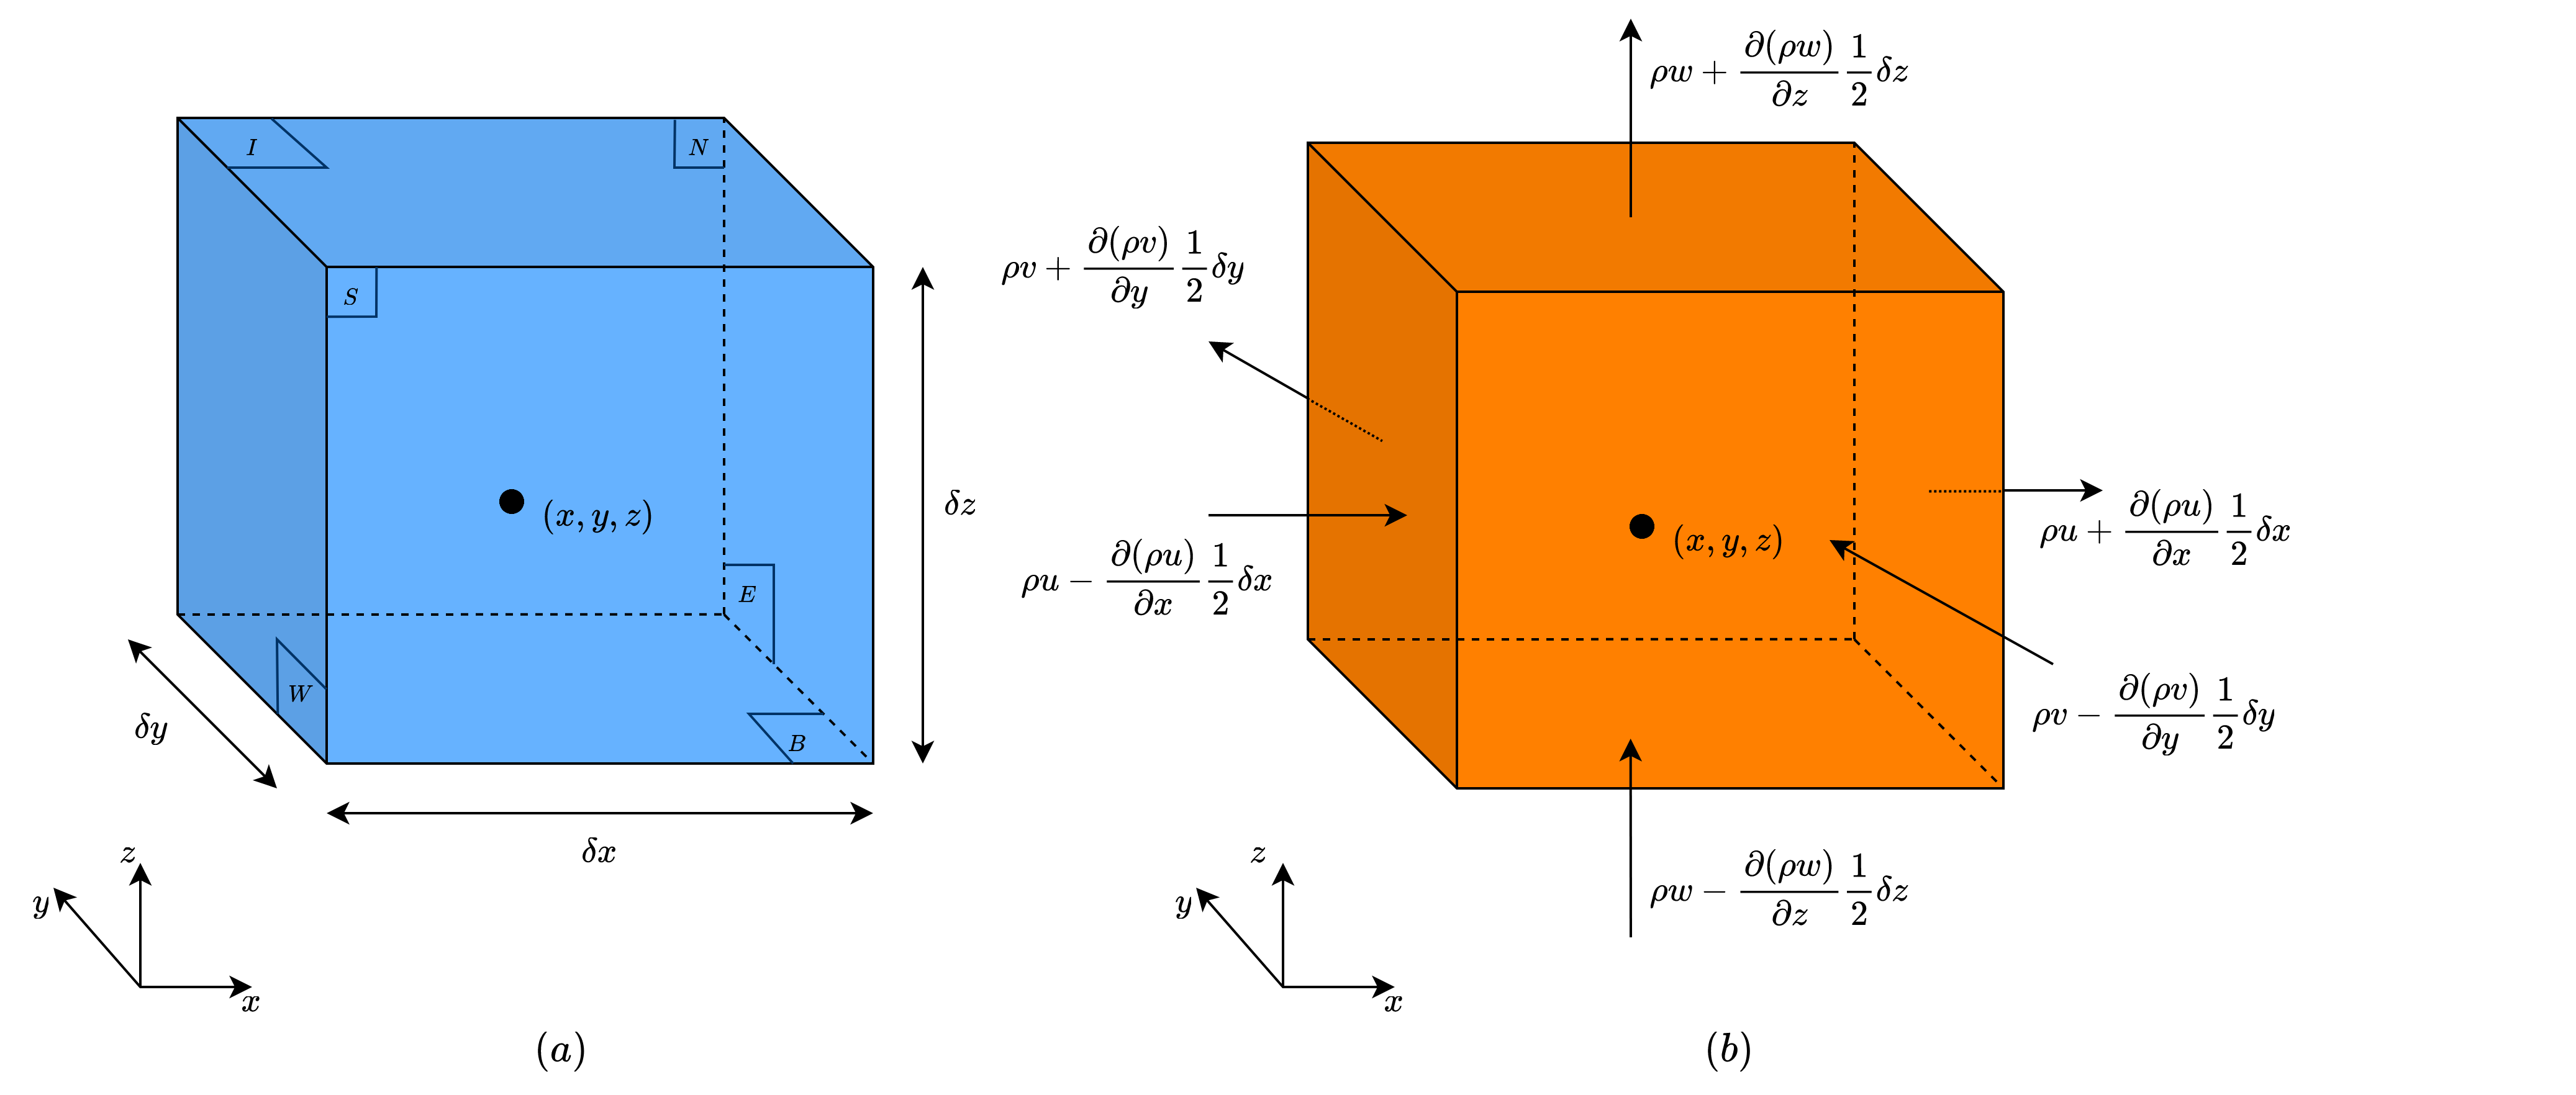
\includegraphics[width=16cm]{contents/cube}
		\caption{(a) Ilustrasi partikel sebagai sifat fisis fluida. (b) Aliran massa jenis masuk dan keluar \protect\shortcite{versteeg2007introduction}}
		\label{fig:cube}
		\medspace
		\small
		Massa jenis dari partikel $\rho(x,y,z,t)$ pada gambar bagian (a) dapat diterjemahkan sebagai aliran yang masuk dan keluar. Pada gambar bagian (b), arah aliran massa jenis pada partikel pusat merupakan jumlahan dari aliran massa jenis masuk dan keluar. Dengan cara yang sama, dapat juga dilakukan untuk tekanan dan kecepatan. 
	\end{figure}
	
\end{spacing}
\vspace{-1pc}
\section[Persamaan Navier-Stokes 3 Dimensi]{Persamaan Navier-Stokes 3 Dimensi}
\begin{spacing}{1.5}
	\par Model sirkulasi laut atau \textit{Ocean General Circulation Models} (OGCM) menggunakan persamaan Navier-Stokes untuk memodelkan fenomena fisis yang terjadi di lautan. Persamaan gerak Navier-Stokes nonhidrostatik dalam model 3-D terdiri dari persamaan momentum, persamaan kontinuitas, dan persamaan konservasi densitas \shortcite{Haditiar2020}. Pada model Navier-Stokes dengan pendekatan nonhidrostatik, tekanan air laut (P) dipecah menjadi dua bagian utama, yaitu: tekanan hidrostatik (p) dan tekanan nonhidrostatik (q)
	\begin{equation}
		P = p+q.
	\end{equation}
	Tekanan p dihitung secara diagnostik dari densitas  dan percepatan gravitasi g seperti pada persamaan berikut 
	\begin{equation}
		\frac{\partial p}{\partial z} = -(\rho - \rho_0)g.
	\end{equation}
	Sedangkan tekanan q dihitung secara prognostik dalam persamaan momentum (implisit). Hal ini karena tekanan q bergantung terhadap sirkulasi arus.
	\par Persamaan momentum lengkap untuk model nonhidrostatik adalah sebagai berikut
	\begin{equation}
		\begin{aligned}
			\frac{\partial u}{\partial t} + \text{adv}(u)-fv &= \frac{-1}{\rho_0}\frac{\partial(p+q)}{\partial x}+\text{diff}(u) \\
			\frac{\partial v}{\partial t} + \text{adv}(v)+fu &= \frac{-1}{\rho_0}\frac{\partial(p+q)}{\partial y}+\text{diff}(v) \\
			\frac{\partial w}{\partial t} +\text{adv}(w) &= \frac{-1}{\rho_0}\frac{\partial(q)}{\partial y}+\text{diff}(w).
		\end{aligned}	
	\end{equation}
	\par Dengan $\text{adv}(\psi)=u\frac{\partial \psi}{\partial x}+v\frac{\partial \psi}{\partial y}+w\frac{\partial \psi}{\partial z}$ adalah persamaan adveksi dan $\text{diff}(\psi)=\frac{\partial}{\partial x}(A_{H} \frac{\partial \psi}{\partial x})+\frac{\partial}{\partial y}(A_{H} \frac{\partial \psi}{\partial y})+\frac{\partial}{\partial z}(A_{Z} \frac{\partial \psi}{\partial z})$ adalah persamaan difusi dengan $A_H$ dan $A_Z$ koefisien gesekan eddy horizontal dan vertikal. 
	\par Kecepatan arus dalam sistem koordinat Cartesian 3-D didefinisikan dengan u,v, dan w. Waktu didefinisikan dengan t, parameter Coriolis dengan f, dan densitas air laut referensi dengan $\rho_0$.
	Untuk persamaan kontinuitas atau kekekalan volume diekspresikan dalam persamaan berikut
	\begin{equation}
		\frac{\partial u}{\partial t} + \frac{\partial v}{\partial t} + \frac{\partial w}{\partial t} = 0.
	\end{equation}
	Berdasarkan persamaan kontinuitas (2.4), tekanan dinamis pada lapisan permukaan dapat dihitung dengan persamaan berikut
	\begin{equation}
		\frac{\partial q_s}{\partial t} = \rho_0 g_i \times \left( \frac{(\partial \left(H \langle u \rangle \right)} {\partial x} + \frac{(\partial \left(H \langle v \rangle \right)} {\partial y}\right)
	\end{equation}
	dengan $q_s = \rho_0 g \eta$. Disini $\rho_0$ adalah densitas air laut referensi, dan $\eta$ adalah elevasi permukaan laut, $H$ adalah total kedalaman laut, dan $< >$ adalah operator rata-rata vertikal.
	\par Densitas air laut bergantung pada temperatur, salinitas, dan tekanan. Selanjutnya asumsikan bahwa air laut hanya bergantung linear terhadap temperatur dan salinitas, serta difusifitas \textit{eddy} untuk temperatur dan salinitas sama. Persamaan konservasi densitas diberikan oleh,
	\begin{equation}
		\frac{\partial \rho}{\partial t} + \text{adv}(\rho) = \text{diff}(\rho).
	\end{equation}
	Dalam aplikasinya, persamaan Navier-Stokes tidak hanya digunakan untuk memodelkan laut, tapi juga merambah ke bidang pemodelan cuaca \shortcite{Rohli2021}, aliran air dalam pipa \shortcite{Ouchiha2012} dan aliran udara di sekitar sayap pesawat \shortcite{Tulus2019}. Dalam bentuk persamaan lengkap dan simplifikasi, persamaan ini juga dapat digunakan untuk mendesain kereta api \shortcite{Croquer2020}, pesawat terbang \shortcite{Chau2021}, dan mobil \shortcite{Ambarita2018}. Terdapat juga studi tentang aliran darah \shortcite{Gill2021}, desain stasiun pembangkit listrik \shortcite{Yang2019}, dan analisis polusi udara \shortcite{Issakhov2022}. 
\end{spacing}
\vspace{-0.1pc}
\section[Model Iklim]{Model Iklim}
\begin{spacing}{1.5}
\end{spacing}
	

%=====================================================================
% BAB III
\chapter{METODOLOGI PENELITIAN}
\vspace{1.5pc}
\section[Domain Penelitian]{Domain Penelitian}
\begin{spacing}{1.5}
	Domain dalam penelitian ini meliputi Samudra Hindia, Teluk Benggala, Laut Andaman, dan Selat Malaka dengan koordinat $0^\circ-24.6^\circ$ LU dan $76.96^\circ-104.96^\circ$ BT (lihat Gambar \ref{fig:domain}). Partikel mikroplastik disimulasikan dengan mengambil titik awal (\textit{starting point}) di beberapa lokasi perairan Aceh untuk melihat sebaran sampah plastik yang dibuang ke laut pada lokasi penelitian. 
	\begin{figure}[H]
		\centering
		\includegraphics[width=15cm]{contents/area_of_interest}
		\caption{Domain Penelitian}
		\label{fig:domain}
		\medspace
		\small
		Domain di plot dengan menggunakan data batimetri pada \href{https://www.naturalearthdata.com/}{https://www.naturalearthdata.com/} dengan skala resolusi 1:10m dari SRTM30+ dan dengan menggunakan library \href{https://scitools.org.uk/cartopy/docs/latest/getting_started/index.html#}{cartopy}, \href{https://matplotlib.org/}{matplotlib}, dan \href{https://seaborn.pydata.org/}{seaborn} dalam Python.
		
	\end{figure}
\end{spacing}
\section[Data Penelitian]{Data Penelitian}
\begin{spacing}{1.5}
\vspace{-1pc}
\subsection[Batimetri]{Batimetri}
	SRTM30+ adalah data digital model elevasi global (DEM) yang diperoleh dari radar SRTM (\textit{Instrument Shuttle Radar Topography}) untuk topografi darat dan ICESat (\textit{Ice, Cloud, and land Elevation SATellite}) untuk topografi es. Batimetri laut didasarkan dari model satelit graivitasi baru dimana rasio gravitasi-topografi dikalibrasi dengan menggunakan 298 juta suara yang diedit \shortcite{Becker2009}.
	\par Resolusi data SRTM30+ setiap spasial 1 arc-second pada bidang lintang dan bujur setara dengan 30 meter pada bidang ekuator (30 arc-second setara dengan 1 kilometer). Data batimetri dari Natural Earth Data menggunakan data SRTM30+ untuk menghasilkan peta dengan resolusi 10m (sangat detail), 50m (detail sedang), dan 110m (detail kasar). Peta Batimetri \ref{fig:domain} dalam penelitian ini menggunakan data resolusi 10m yang dapat didownload di \href{https://www.naturalearthdata.com/downloads/10m-physical-vectors/10m-bathymetry/}{https://www.naturalearthdata.com/}.
\subsection[Data NEMO]{Data NEMO}
	Penelitian ini menggunakan data output model NEMO (\href{https://www.nemo-ocean.eu/}{https://www.nemo-ocean.eu/}) untuk data analisis global arus tiga dimensi yang didownload dari website \href{https://resources.marine.copernicus.eu/products}{CMEMS} dari April 2021 - Maret 2022.  Dalam analisis kami, resolusi data output yang digunakan adalah dx = dy = 5 menit pada bidang horizontal dan 50-lapisan $(k \in [1,50])$ dengan ketebalan berbeda pada bidang vertikal:
	\begin{equation*}
		\begin{aligned}
			z_k = \{0.49, 1.54, 2.65, 3.82, 5.08, 6.44, 7.93, 9.57, 11.40, 13.47, 15.82, 18.50, \\
			21.60, 25.21, 29.44, 34.43, 40.34, 47.37, 55.76, 65.81, 77.85, 92.33, 109.73, 130.67, \\
			155.85, 186.12, 222.47, 266.04, 318.13, 380.21, 453.94, 541.089, 643.57, 763.33, \\
			902.34, 1062.44, 1245.29, 1452.25, 1684.28, 1941.89, 2225.08, 2533.33, 2865.70,  \\
			3220.82, 3597.03, 3992.48, 4405.22, 4833.29, 5274.78, 5727.92 \} (m). \\
		\end{aligned}
	\end{equation*}
	\par Model NEMO atau \textit{Nucleus for European Modeling of the Ocean} adalah model komputasi resolusi tinggi yang digunakan untuk kegiatan penelitian dan layanan peramalan dalam oseanografi dan klimatologi, yang dikembangkan secara berkelanjutan sejak tahun 2008 oleh konsorsium Eropa yang terdiri dari 5 institusi (CMCC | CNRS | Mercator Ocean | Met Office | NERC). Hal ini dimaksudkan untuk menjadi alat yang fleksibel untuk mempelajari fenomena fisik dan biogeokimia dalam sirkulasi laut, serta interaksinya dengan komponen sistem iklim Bumi, pada berbagai skala ruang dan waktu \cite{madec_gurvan_2022_6334656}.
\subsection[Data HYCOM]{Data HYCOM}
	Data HYCOM digunakan sebagai data perbandingan dalam penelitian ini. HYCOM (\textit{HYbrid Coordinate Ocean Model}) (\href{https://www.hycom.org}{https://www.hycom.org}) adalah salah satu model sirkulasi laut (OGCM) yang menggunakan model numerik tiga dimensi Navier-Stokes dengan input data batimetri dari GEBCO (\textit{General Bathymetric Chart of the Oceans}), data asimilasi hidrografi laut dari NCODA (\textit{Navy Coupled Ocean Data Assimilation}) dan komponen meteorologi dari NCEP (\textit{National Centers for Environmental Prediction}) ataupun NAVGEM (\textit{The NAVy Global Environmental Model}) berupa angin, kecepatan, fluks panas, tekanan permukaan laut, presipitasi, temperature, dan kelembapan \shortcite{JosephMetzger2013}. Koordinat vertikal dalam HYCOM adalah isopiknal di lautan terbuka yang terstratifikasi dan memiliki transisi yang mulus dan dinamis serta bergantung terhadap waktu pada medan daerah pesisir yang dangkal dan pada tingkat tekanan tetap di lapisan campuran permukaan atau lautan yang tidak terstratifikasi \shortcite{chassignet2017,Park2013}. 
	\par Data HYCOM yang digunakan adalah data analisis global arus tiga dimensi dengan resolusi spasial 5 menit untuk longitude dan 2.5 menit untuk latitude selama setahun (April 2021 - Maret 2022) dan dengan ketebalan bervariasi pada bidang vertikal, yaitu 40-lapisan $(k \in [1,40])$:
	\begin{equation*}
		\begin{aligned}
			z_k = \{0.0, 2.0, 4.0, 6.0, 8.0, 10.0, 12.0, 15.0, 20.0, 25.0, 30.0, 35.0, 40.0, 45.0, 50.0, \\
			60.0, 70.0,	80.0, 90.0, 100.0, 125.0, 150.0, 200.0, 250.0, 300.0, 350.0, 400.0, 500.0, 600.0,\\
			700.0, 800.0, 900.0, 1000.0, 1250.0, 1500.0, 2000.0, 2500.0, 3000.0, 4000.0, 5000.0\} (m). \\
		\end{aligned}
	\end{equation*}
\end{spacing}
\vspace{-1.5pc}
\section[Prosedur Penelitian]{Prosedur Penelitian}
\begin{spacing}{1.5}
	\begin{figure}[H]
		\centering
		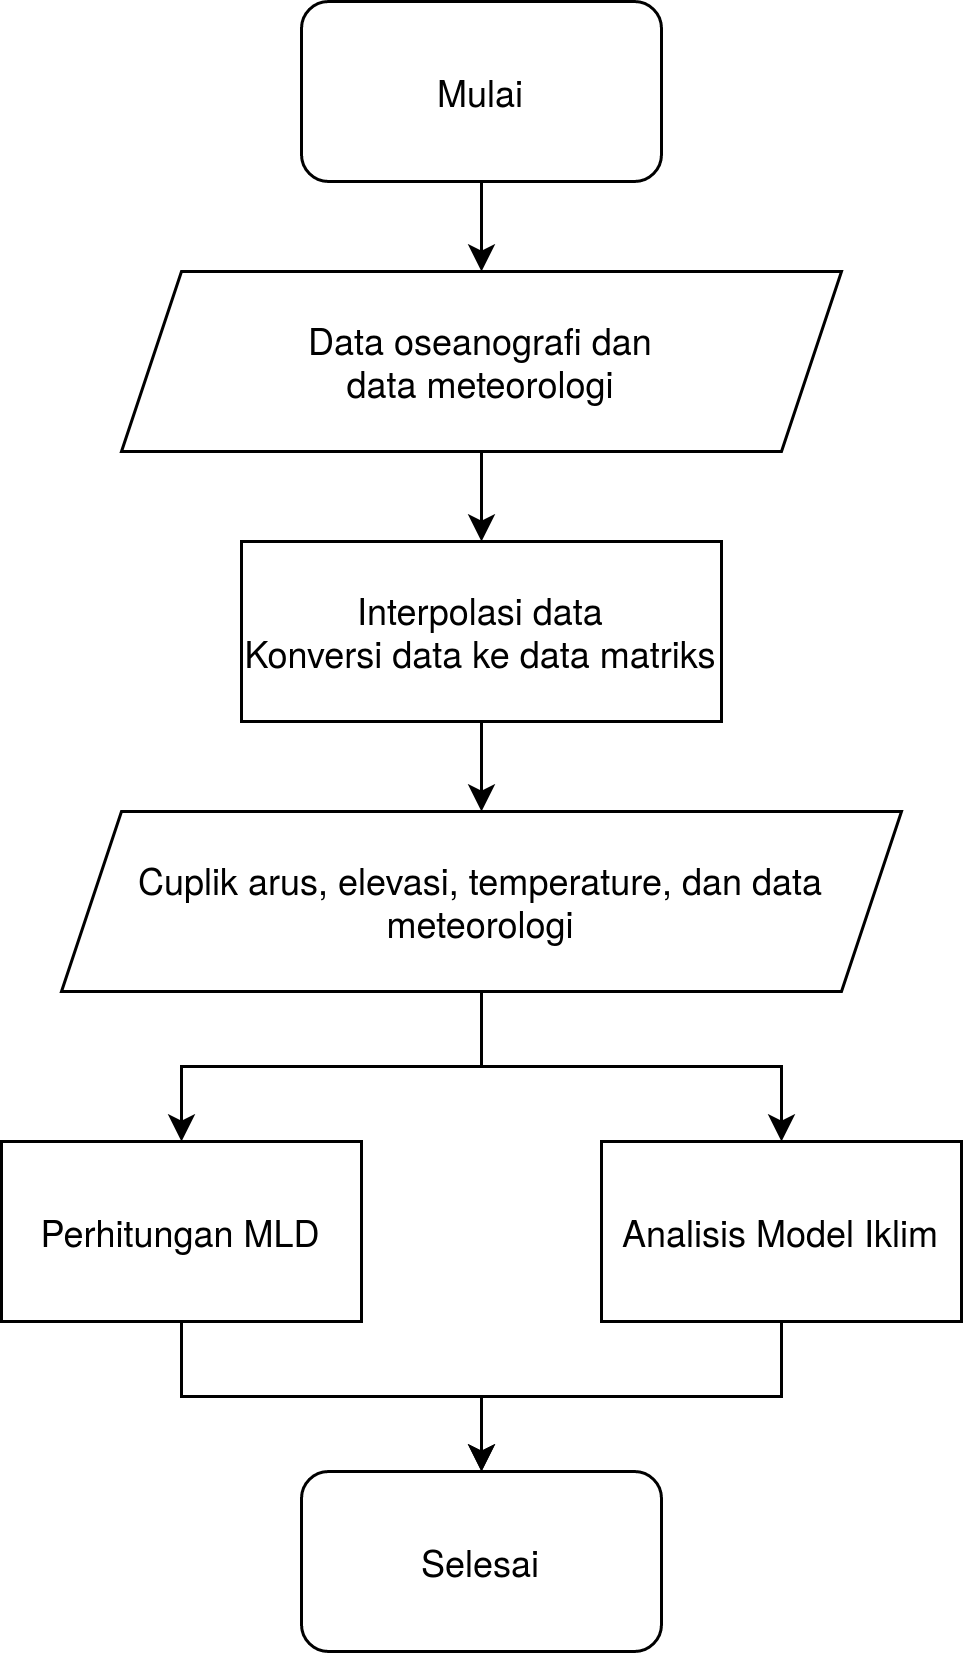
\includegraphics[width=15cm]{contents/flowchart.png}
		\caption{Diagram alir }
		\label{fig:flowchart}
	\end{figure}
	Prosedur penelitian mengikuti diagram alir pada Gambar \ref{fig:flowchart}. Pertama-tama akan dilakukan konfigurasi modul yang ada dalam Python untuk menentukan input langkah waktu simulasi yang digunakan, penentuan lokasi dan  jumlah partikel yang keluar, serta konfigurasi kernel dalam hal ini perlakuan partikel, perilaku, dan lama waktu penelitian. Selanjutnya data-data OGCM yang diperlukan didownload dari situs CMEMS, HYCOM, dan NCEP. Data-data yang telah didownload kemudian diinterpolasi agar sesuai dengan software Parcel yang digunakan dan disimpan dalam data \textit{field}. Setelah kernel didefinisikan dan dikonfigurasi, data \textit{field} kemudian diproses menggunakan algoritma Parcel dan dilakukan perulangan untuk waktu yang terintegrasi, dijalankan bersama dengan modul tambahan secara paralel serta memperbaharui kondisi partikel-partikel, dan menghasilkan output berupa NetCDF atau NumPy array. Langkah terakhir adalah proses analisis dan visualisasi hasil.
\end{spacing}
%=====================================================================
%% Halaman Output
%\pagebreak
%\chapter*{OUTPUT PROPOSAL TESIS}
%\addtocontents{toc}{\begingroup\protect\setlength{\protect\cftsecindent}{-\leftmargin}}
%\addcontentsline{toc}{section}{\protect\numberline{}\textbf{OUTPUT PROPOSAL TESIS}}	
%\addtocontents{toc}{\endgroup}
%\vspace{1.5pc}
\begin{spacing}{1.5}
	Sebagai informasi bahwa proposal ini merupakan awal dari Penelitian Proposal PMDSU (Kesepatan dengan Prof. Dr. Syamsul Rizal dan Prof Dr. Marwan Ramli, S.Si., M.Si.) yang harus saya jalankan, oleh karena itu segala output dari penelitian ini diharapkan mampu memenuhi persyaratan publikasi PMDSU. 
	
	Output dari proposal penelitian ini direncanakan dapat terpublikasi di beberapa konferensi dan jurnal berikut:
	\begin{enumerate}
		\item Output konferensi AIC (Annual International Conference 2022), terindeks scopus.
		\begin{itemize}
			\item Waktu: Deadline submit abstrak 29 Agustus 2022, Konferensi 12-13 Oktober 2022.
			\item Judul (tentatif): \textit{Surface Circulation in Aceh Waters, Malacca Strait, and Part of South China Sea.}
			\item Domain penelitian:
			\begin{figure}[H]
				\centering
				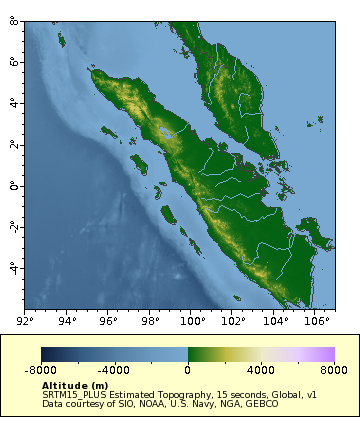
\includegraphics[width=8cm]{contents/srtm15plus}
				\caption{Domain penelitian meliputi: Perairan Aceh, Selat Malaka, dan Bagian Laut Cina Selatan}
			\end{figure}
		\end{itemize}
		\item Output konferensi ICFAES (International Conference on Fisheries, Aquatic, and Environmental Sciences), terindeks scopus.
		\begin{itemize}
			\item Waktu: Deadline submit abstrak 30 Agustus 2022, Konferensi 26 Oktober 2022.
			\item Judul (tentatif): \textit{Monthly analysis of Chlorophyll-a, Sea Surface Temperature, and Sea Surface Salinity in the Bay of Bengal (years 2015-2021).}
			\item Domain penelitian:
			\begin{figure}[H]
				\centering
				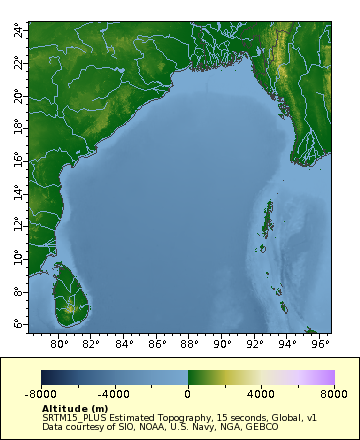
\includegraphics[width=8cm]{contents/srtm15plus_1}
				\caption{Domain penelitian Teluk Benggala}
			\end{figure}
		\end{itemize}
		\item Output jurnal JGR (Journal of Geophysical Research)
		\begin{itemize}
			\item Status: \textit{Submitted} (2022-07-4).
			\item Judul (tentatif): \textit{Effect of Meteorological Parameters on Ocean Layer Variability in the Bay of Bengal.}
			\item Domain penelitian:
			\begin{figure}[H]
				\centering
				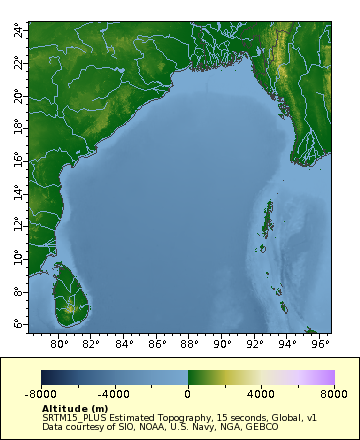
\includegraphics[width=8cm]{contents/srtm15plus_1}
				\caption{Domain penelitian Teluk Benggala}
			\end{figure}
		\end{itemize}
	\end{enumerate}
\end{spacing}
%=====================================================================
 BAB IV
\chapter{HASIL DAN PEMBAHASAN}
%\vspace{1.5pc}
\vspace{1.5pc}
\section[Aplikasi pada \textit{Bay of Bengal}(BoB)]{Aplikasi pada \textit{Bay of Bengal} (BoB)}
\begin{spacing}{1.5}
\vspace{-1pc}
\subsection[Sirkulasi Arus dan Angin]{Sirkulasi Arus dan Angin}
	
	\lipsum[1]

\subsection[Profil Transek Vertikal]{Profil Transek Vertikal}
	
	\lipsum[1]
	
\subsection[Hubungan antara Parameter Meteorologi]{Hubungan antara Parameter Meteorologi}
	
	\lipsum[1]
	

\subsection[Model Iklim]{Model Iklim}
	
	\lipsum[1]
	
\end{spacing}

\section[Aplikasi pada Perairan Aceh]{Aplikasi pada Perairan Aceh}
\begin{spacing}{1.5}
	\vspace{-1pc}
	\subsection[Sirkulasi Arus dan Angin]{Sirkulasi Arus dan Angin}
	
	\lipsum[1]
	
	\subsection[Profil Transek Vertikal]{Profil Transek Vertikal}
	
	\lipsum[1]
	
	\subsection[Hubungan Antara Parameter Meteorologi]{Hubungan Antara Parameter Meteorologi}
	
	\lipsum[1]
	
	
	\subsection[Model Iklim]{Model Iklim}
	
	\lipsum[1]
	
\end{spacing}
%=====================================================================
% BAB V
%\chapter{PENUTUP}
%\vspace{1.5pc}
\vspace{1.5pc}
\begin{spacing}{1.5}
\section[Kesimpulan]{KESIMPULAN}

\lipsum[2-4]

\section[Saran]{SARAN}

\lipsum[2-4]\cite{Adams2011}

\end{spacing}
%=====================================================================
% Halaman Daftar Pustaka
\pagebreak
%\addcontentsline{toc}{chapter}{\textbf{DAFTAR PUSTAKA}}
\renewcommand\bibname{DAFTAR PUSTAKA}	
\bibliographystyle{packages/apacite}
\bibliography{contents/ReferenceMendeley.bib}
%\{DAFTAR}
%=====================================================================
% Halaman Lampiran
\newpage
\newappendix{Lampiran 1. Penjabaran Persamaan Navier-Stokes}
\addcontentsline{toc}{chapter}{LAMPIRAN}
\section*{SIMBOL}
	\begin{tabular}{ll}
		$\alpha$ & Konstanta pergeseran vertikal\\
		$\beta$ & Amplitudo dari gelombang sinus\\
		$\epsilon$ & Elemen residual\\
		$f$ & Parameter Coriolis, dengan $f=2\Omega \cdot k$\\
		$\gamma$ & Amplitudo dari gelombang kosinus\\
		$\Omega$ & Vektor kecepatan sudut bumi \\
		$p$ & Tekanan \\
		$\rho$ & Densitas \\
		$\rho_o$ & Densitas referensi\\
		$r$ & Koefisien korelasi \\
		$S$ & Salinitas\\
		$t$ & Waktu\\
		$T$ & Temperature potensial\\
		$\theta$ & Perpindahan fase\\
		$\omega$ & Kecepatan sudut \\
		$u,v$ & Kecepatan arus\\
		
	\end{tabular}	
\section*{SATUAN}
	\begin{tabular}{ll}
		$^\circ$C & Derajat Celcius \\
		$^\circ \text{C jam}^{-1}$ & Derajat Celcius per jam\\
		$kg/kg$ & Kilogram per kilogram\\
		$kg/m^2s$ & Kilogram per meter persegi \textit{second}\\
		$kPa$ & Kilo Pascal\\
		$m$ & Meter\\
		$m/s$ & Meter per \textit{second}\\
		$Pa$ & Pascal\\
		PSU & \textit{Practical salinity unit} \\
		$Wm^{-2}$ & Watt per meter persegi\\
		
	\end{tabular}

\section*{AKRONIM}
	\begin{tabular}{ll}
		3-D & Dimensi 3\\
		AirT & \textit{2m Air temperature}\\
		BoB & \textit{Bay of bengal}\\
		BT & Bujur timur\\
		Chl-a & \textit{Chlorophyll-a}\\
		CMCC & \textit{Centro Euro-Mediterraneo sui cambiamenti climatici}\\
		CMEMS & \textit{Copernicus Marine Environment Monitoring Service}\\
		CNRS & \textit{Centre national de la recherche scientifique}\\
		CPrecR & \textit{Convective precipitation rate}\\
		EICC & \textit{East India coastal current}\\
		GEBCO & \textit{General bathymetric chart of the oceans}\\
		HYCOM & \textit{HYbrid coordinate ocean model}\\
		ILD & \textit{Isothermal layer depth}\\
		LU & Lintang utara\\
		MET office & \textit{Meteorological office}\\
		MLD & \textit{Mixed layer depth}\\
		MODIS & \textit{Moderate resolution imaging spectroradiometer}\\
		NAVGEM & \textit{NAVy global environmental model}\\
		NCEP/NCAR & \textit{National centers for environmental prediction/} \\
		& \textit{National center for atmospheric research}\\
		NCODA & \textit{Navy coupled ocean data assimilation}\\
		NEMO & \textit{Nucleus for European modelling of the ocean}\\
		NERC & \textit{Natural environment research council}\\
		ND & \textit{Net deployment}\\
		OGCM & \textit{Ocean general circulation model}\\
		RMSE & \textit{Root mean square error} \\
		RW & \textit{Relative wind}\\
		SCM & \textit{Subsurface chlorophyll-a maximum}\\
		SHum & \textit{2m Specific Humidity}\\
		SLP & \textit{Sea level pressure}\\
		SRTM15+ & \textit{Shuttle radar topography mission 15 arc seconds}\\
		SSH & \textit{Sea surface height} \\
		SSS & \textit{Sea surface salinity} \\
		SST & \textit{Sea surface temperature}\\
		TCHP & \textit{Tropical cyclone heat potential} \\
		Qnet & \textit{Net surface heat flux} \\
		WHOI & \textit{Woods hole oceanographic institution} \\
		TauX & \textit{Wind stress U}\\
		TauY & \textit{Wind stress V}\\
	\end{tabular}
%\section*{ISTILAH}
%\begin{tabular}{ll}
%	$^\circ$C & Derajat Celcius \\
%	$m$ & Meter\\
%	$m/s$ & Meter per \textit{second}\\
%	$Pa$ & Pascal\\
%	PSU & \textit{Practical salinity unit} \\
%	$Wm^{-2}$ & Watt per meter persegi\\
%	$^\circ \text{C jam}^{-1}$ & Derajat Celcius per jam\\
%\end{tabular}
%\pagebreak
%\newappendix{Lampiran 2. Diskritisasi pada C-grid Arakawa}
%\begin{spacing}{1.5}
	\begin{figure}[H]
		\centering
		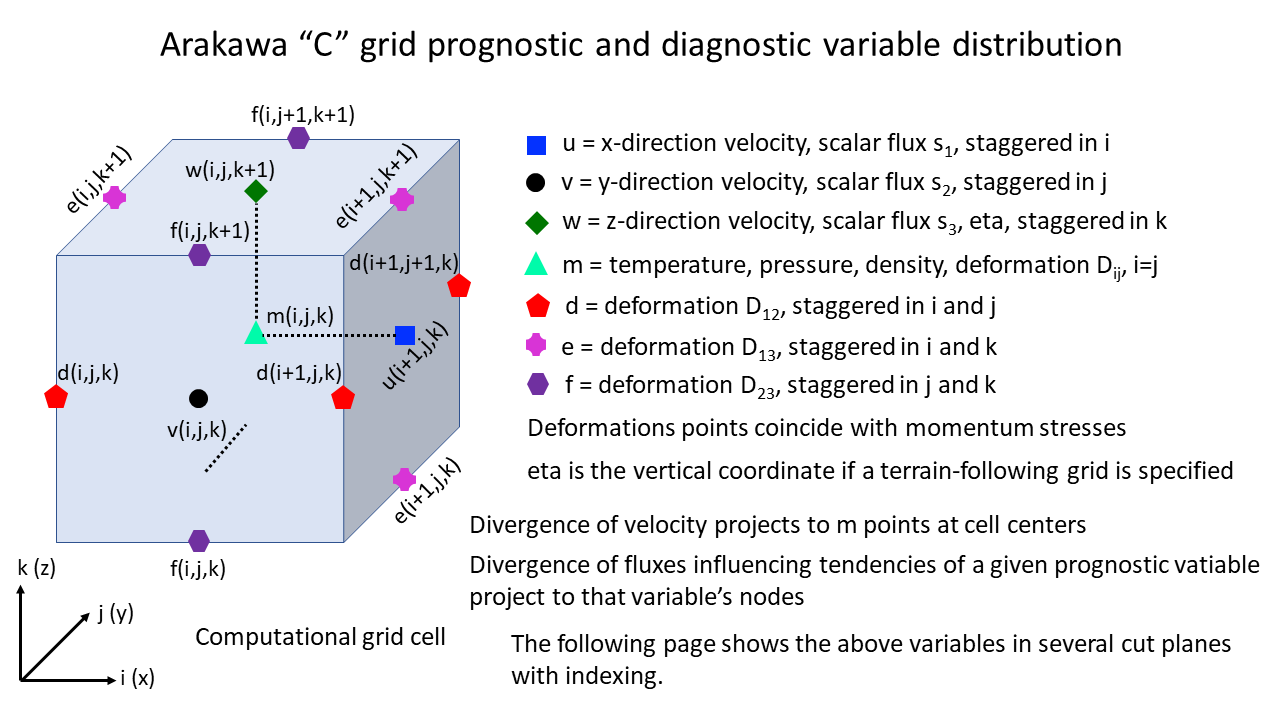
\includegraphics[width=1\textwidth]{contents/Arakawa_1.png}		
		\caption{Distribusi variabel pada C-grid Arakawa}
		\label{fig:arakawa_1}
	\end{figure}
	\begin{figure}[H]
		\centering
		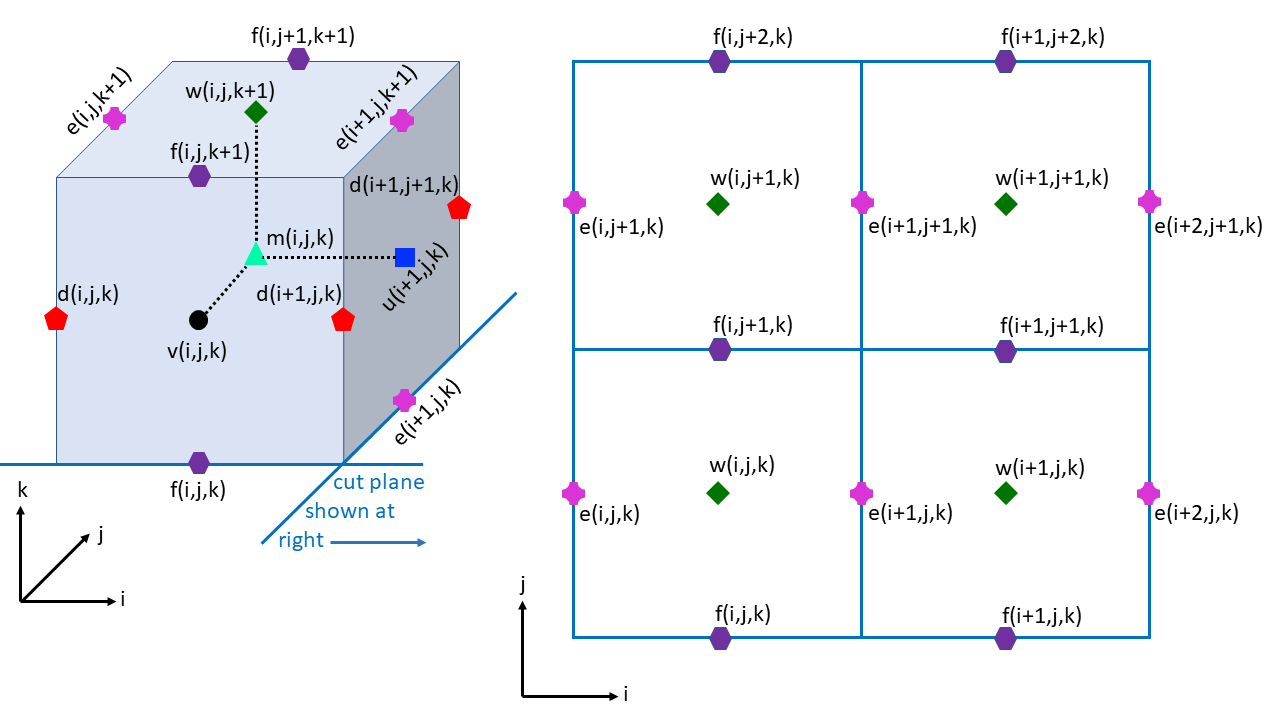
\includegraphics[width=1\textwidth]{contents/Arakawa_2.png}	
		\caption{Diskritisasi C-grid Arakawa (posisi bawah kubus, $k$ tetap)}
		\label{fig:arakawa_2}
	\end{figure}
	\begin{figure}[H]
		\centering
		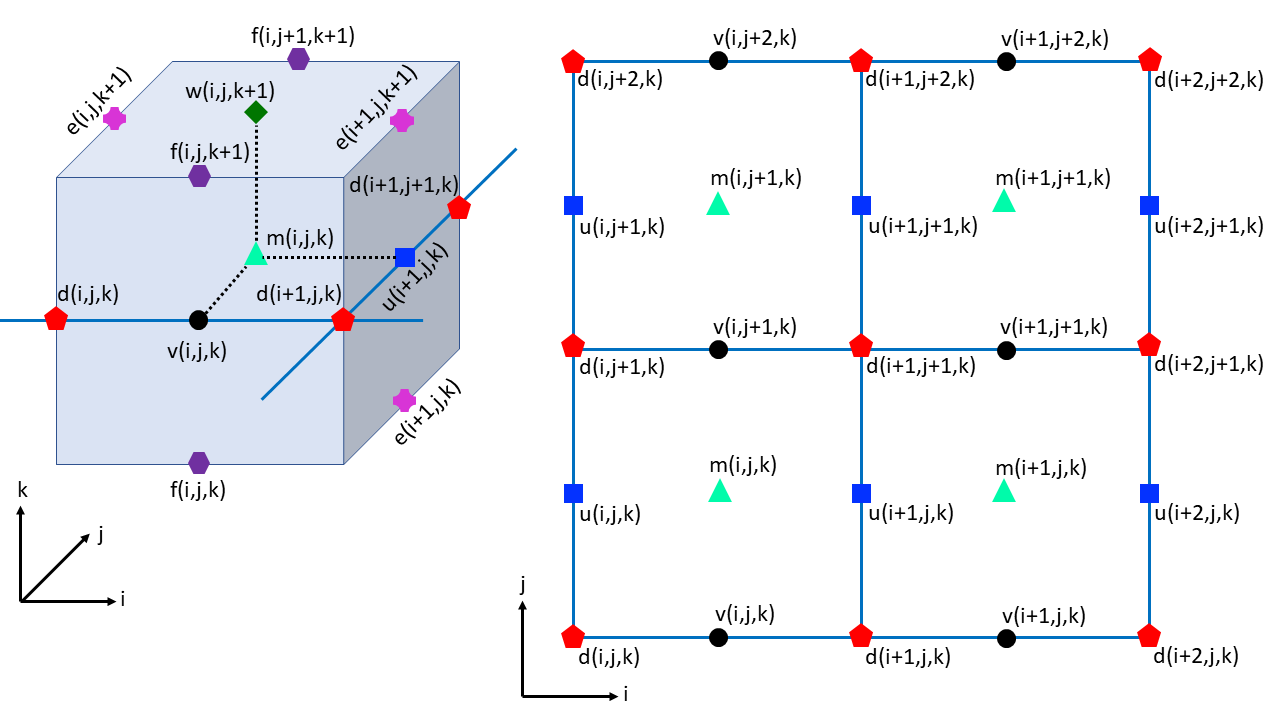
\includegraphics[width=1\textwidth]{contents/Arakawa_3.png}	
		\caption{Diskritisasi C-grid Arakawa (posisi tengah kubus, $k$ tetap)}
		\label{fig:arakawa_3}
	\end{figure}
		\begin{figure}[H]
		\centering
		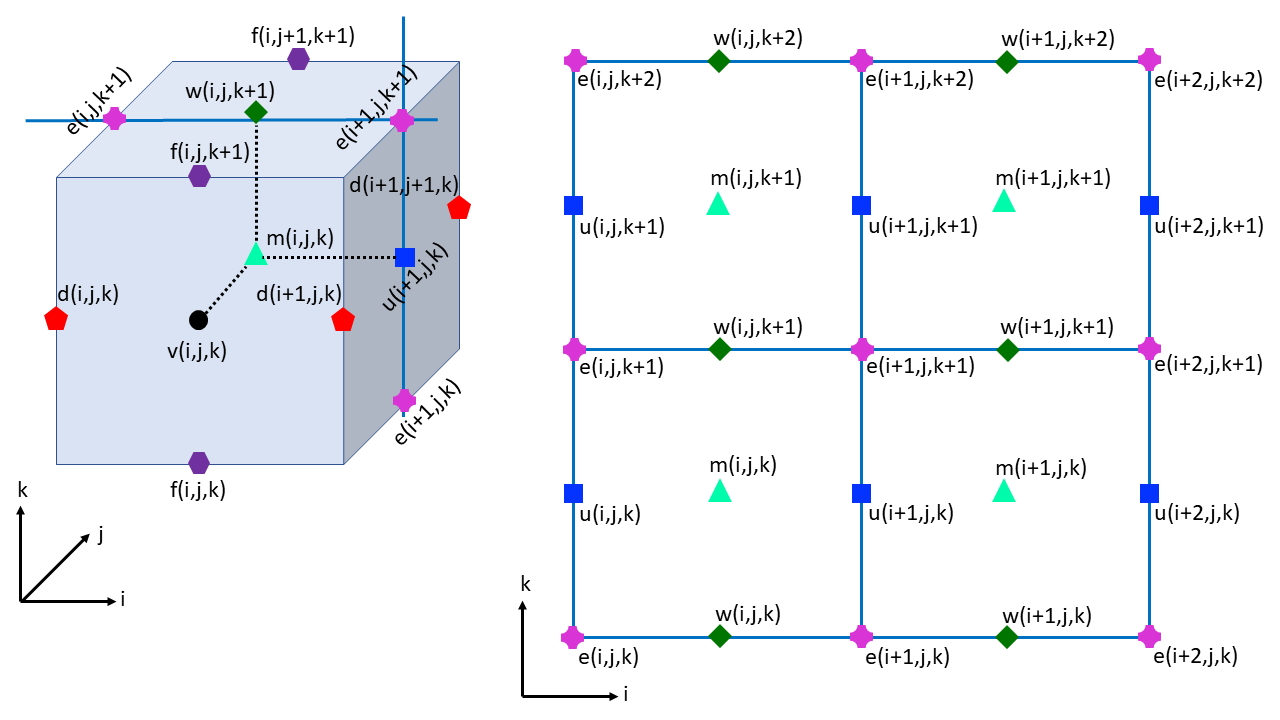
\includegraphics[width=1\textwidth]{contents/Arakawa_4.png}	
		\caption{Diskritisasi C-grid Arakawa ($j$ tetap)}
		\label{fig:arakawa_4}
	\end{figure}
		\begin{figure}[H]
		\centering
		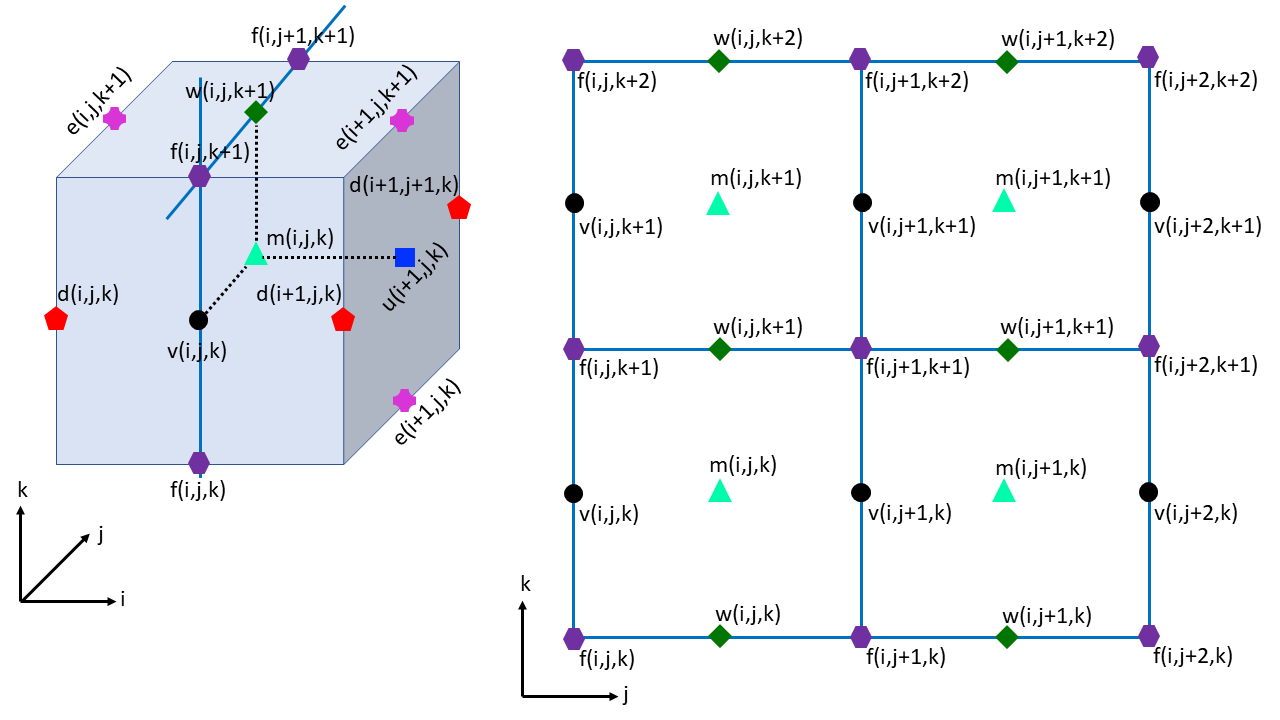
\includegraphics[width=1\textwidth]{contents/Arakawa_5.png}	
		\caption{Diskritisasi C-grid Arakawa ($i$ tetap)}
		\label{fig:arakawa_5}
	\end{figure}
\end{spacing}
%\pagebreak
%\newappendix{Lampiran 3.}
%\begin{figure}[H]
	\centering
	\includegraphics[width=15cm]{contents/final_figure/SeasonalModel9}
	\caption{\textit{Seasonal model} pada latitude 9$^\circ$C untuk (a) 2m \textit{air temperature},(b) 2m \textit{specific humidity},(c) \textit{Convective precipitation rate},(d) \textit{Sea level pressure},(e) \textit{Wind stress U},(f) \textit{Wind stress V}}
	\label{fig:SM9}
\end{figure}

\begin{figure}[H]
	\centering
	\includegraphics[width=15cm]{contents/final_figure/SeasonalModel19}
	\caption{\textit{Seasonal model} pada latitude 19$^\circ$C untuk (a) 2m \textit{air temperature},(b) 2m \textit{specific humidity},(c) \textit{Convective precipitation rate},(d) \textit{Sea level pressure},(e) \textit{Wind stress U},(f) \textit{Wind stress V}}
	\label{fig:SM19}
\end{figure}

\begin{figure}[H]
	\centering
	\includegraphics[width=15cm]{contents/final_figure/MLD_Part1}
	\caption{Peta MLD untuk bulan (a) Januari, (b) Februari, (c) Maret, (d) April, (e) Mei, dan (f) Juni}
	\label{fig:MLD_part1}
\end{figure}

\begin{figure}[H]
	\centering
	\includegraphics[width=15cm]{contents/final_figure/MLD_Part2}
	\caption{Peta MLD untuk bulan (g) Juli, (h) Agustus, (i) September, (j) Oktober, (k) November, dan (l) Desember}
	\label{fig:MLD_part2}
\end{figure}
%=====================================================================
% Halaman Biodata
%\newpage
%\chapter*{BIODATA}
%\vspace{1.5pc}
\vspace{1.5pc}
\begin{spacing}{1.5}
\thispagestyle{empty}
\begin{flushleft}
\begin{tabular}{lp{0.25cm}p{9cm}}
Nama &:& Harish Abdillah Mardi\\
Tempat, tanggal lahir &:& Banda Aceh, 03 April 1999\\
Alamat &:& Komplek Dosen Desa Blangkrueng No.86, Baitussalam, Kabupaten Aceh Besar\\
Nama Ayah &:& Marwan\\
Pekerjaan Ayah &:& Dosen\\
Nama Ibu &:& Dian Mawarni\\
Pekerjaan Ibu &:& Ibu rumah Tangga\\	
Alamat Orang Tua &:& Komplek Dosen Desa Blangkrueng No.86, Baitussalam, Kabupaten Aceh Besar\\
\end{tabular}
\end{flushleft}

\noindent\hspace{0.1cm} Riwayat pendidikan :

\begin{table}[ht]
\centering
\vspace{0.1cm}
\begin{tabular}{|p{1.5cm}|p{5.3cm}|p{3cm}|p{1.5cm}|c|c|c|c|c|c|c|c|c|c|c|c|c|c|c|c|c|}
    \hline
   \centering \multirow{2}{*}{Jenjang} & \centering \multirow{2}{*}{Nama Sekolah} & \centering \multirow{2}{*}{Bidang Studi} & \multirow{2}{*}{Tempat} & Tahun\\
    &&&&Ijazah\\
    \hline
     \centering   SD&SD Swasta Sutomo 1 Medan&\centering -&\centering Medan&2011\\
    \hline
      \centering  SMP&SMP Swasta Sutomo 1 Medan&\centering -&\centering Medan&2014\\
    \hline
       \centering\multirow{2}{*}{SMA} &SMA Swasta Husni Thamrin Medan &\centering\multirow{2}{*}{IPA} &\centering\multirow{2}{*}{Medan}&\multirow{2}{*}{2017}\\
    \hline
        \centering Sarjana (S1)&Jurusan Fisika, Fakultas MIPA, Universitas Syiah Kuala & \centering Fisika Teori dan Komputasi&\centering Banda Aceh&\multirow{2}{*}{2021}\\
    \hline
\end{tabular}
\end{table}

\noindent\hspace{0.1cm} Karya tulis yang pernah dihasilkan :

\begin{table}[ht]
\centering
\vspace{0.1cm}
\begin{tabular}{|p{0.5cm}|p{7.7cm}|p{1cm}|c|}
    \hline
         \centering   No & \centering Judul & \centering Tahun & Penerbit\\
    \hline
   \centering \multirow{4}{*}{1} & Pemodelan Dispersi Gelombang pada Medium & \centering \multirow{4}{*}{2021} &\\
    &  Fiber Optik Berdasarkan Persamaan Nonlinier&& FMIPA,\\
    &   Schr\"odinger (NLS) && UNSIYIAH\\
    & (Tugas Akhir/Skripsi) &&\\
    \hline
\end{tabular}
\end{table}
\end{spacing}
%=====================================================================
\end{document}
